\documentclass[conference]{IEEEtran}
\IEEEoverridecommandlockouts
% The preceding line is only needed to identify funding in the first footnote. If that is unneeded, please comment it out.
\usepackage{cite}
\usepackage{amsmath,amssymb,amsfonts}
\usepackage{algorithmic}
\usepackage{graphicx}
\usepackage{textcomp}
\usepackage[OT1]{fontenc}
\usepackage{xcolor}
\usepackage{multirow,makecell,booktabs}
\usepackage{adjustbox,threeparttable}
\newtheorem{theorem}{Theorem}[section]
\newtheorem{lemma}[theorem]{Lemma}

\ifCLASSOPTIONcompsoc
\usepackage[caption=false, font=normalsize, labelfont=sf, textfont=sf]{subfig}
\else
\usepackage[caption=false, font=footnotesize]{subfig}
\fi
% \usepackage[colorlinks]{hyperref}
\def\BibTeX{{\rm B\kern-.05em{\sc i\kern-.025em b}\kern-.08em
    T\kern-.1667em\lower.7ex\hbox{E}\kern-.125emX}}
\begin{document}

\title{Privacy-Preserving Truth Discovery for Sparse Data in Mobile Crowdsensing Systems\\
% \title{Privacy-preserving truth discovery in sparse mobile crowd sensing systems\\
% {\footnotesize \textsuperscript{*}Note: Sub-titles are not captured in Xplore and
% should not be used}
% \thanks{Identify applicable funding agency here. If none, delete this.}
}


\author{\IEEEauthorblockN{Feng Liu, Bin Zhu, Shaoxian Yuan, Kaiping Xue$^\dag$}
\IEEEauthorblockA{School of Cyber Security, University of Science and Technology of China, Hefei, Anhui 230027, China\\
$^\dag$Corresponding author, kpxue@ustc.edu.cn
% \textit{University of Science and Technology of China}\\
% Hefei, Anhui 230027, China \\
}
}

\maketitle

\begin{abstract}
Truth discovery is an effective method to infer truthful information from a large amount of sensory data in mobile crowdsensing systems.
Privacy-preserving truth discovery schemes require the cloud server not to access each worker's sensory data directly so that the privacy of sensory data can be preserved.
In some specific applications such as sparse mobile crowdsensing, workers can only contribute sensory data on a small part of sensing tasks, implying that the information of which tasks are completed by a worker should also be preserved.
 % which implies that the information of 
% . This implies that the information of which tasks are completed by a worker should also be protected.
% whether or not a worker collects specific data should also be protected.
% the sensory data collected by workers are usually sparse, which implies that the information of whether or not a worker collects specific data should also be protected.
% In real practice such as sparse crowdsensing, it is common that the sensory data collected by some participants are sparse, which implies that the privacy of whether or not a participant collects specific data also needs to be protected.
However, existing privacy-preserving truth discovery schemes do not consider such sparse data scenarios in mobile crowdsensing systems.
In this paper, we first identify the privacy issues in truth discovery when sensory data are sparse.
To address these issues, we design a privacy-preserving truth discovery scheme by employing the additively homomorphic cryptosystem and additive secret sharing with two non-colluding servers.
Through detailed analysis and extensive experiments, we demonstrate that our proposed scheme can satisfy strong privacy-preserving requirements with low computation and communication overhead.
\end{abstract}
\begin{IEEEkeywords}
Truth Discovery, Privacy Preservation, Sparse Data, Mobile Crowdsensing
\end{IEEEkeywords}

\section{Introduction}~\label{sec1}
Over the past few years, developments in the field of cloud computing and the Internet of Things have led to a growing interest in mobile crowdsensing systems.
In a typical mobile crowdsensing system, the cloud server can analyze the sensory data provided by a number of mobile devices (usually referred to as {\em workers}, e.g., smartphones, wearables, and on-board computers).
Since the quality of sensory data provided by different workers may vary greatly, how to derive the truthful information from sensory data of different qualities becomes a major obstacle.
To address this challenge, an effective method called truth discovery~\cite{li_resolving_2014,li_confidence-aware_2014,li_conflicts_2016} was proposed, where the general principle is to calculate each worker's reliability degree (usually referred to as {\em weight}) before estimating the truths.

Although truth discovery can help cloud server to derive truthful information in an effective way, it poses threats to workers' privacy directly.
Several researchers~\cite{miao_cloud-enabled_2015,xu_efficient_2019,miao_lightweight_2017,zhang_reliable_2019,xue_inpptd_2020,tang_achieving_2021} pointed out that the data provided by workers are sensitive to some extent, and designed diverse privacy-preserving truth discovery schemes to assure workers' privacy.
% have been developed to assure workers' privacy.
% To assure sensory data privacy, several works~\cite{miao_cloud-enabled_2015,miao_lightweight_2017,xu_efficient_2019,zhang_reliable_2019,xue_inpptd_2020} have been proposed by utilizing different approaches.
These works mainly focus on the privacy of workers' sensory data, and some of them (such as~\cite{zhang_reliable_2019,xue_inpptd_2020,tang_achieving_2021}) further argued that the privacy of workers' weights should also be preserved.
% 以上方案没有考虑两类问题: 如何处理稀疏的感知数据, 稀疏情况下又带来什么安全问题
So far, these schemes can only be applied to the situation where workers have to execute all sensing tasks.
 % provide sensory data for the whole sensing tasks.
However, due to the variety of task types and workers' abilities, requiring each worker to execute all sensing tasks seems unrealistic.
Especially in the mobile crowdsensing systems, it is quite common that a worker only executes partial tasks for saving energy~\cite{wang_sparse_2016,wang_energy_2018}.
Under these circumstances, the sensory data provided by workers probably are only concerned with partial sensing tasks, namely, the sensory data are sparse.
To the best of our knowledge, there has been little discussion about privacy-preserving truth discovery in such a sparse data environment.
% However, far too little attention has been paid to the situation where sensory data provided by workers are sparse.
% However, 
% workers' observed objects are incomplete.
% However, only taking the privacy of sensory data and weights into account is not sufficient on the situation where the sensory data provided by workers are sparse.
% Fig presents the example of sparse mobile crowdsensing~\cite{wang_sparse_2016}, in which the sensed objects represent different subareas of a city.
% To collect sensory data for all sensed objects, workers need to access all distinct subareas in the city within a specific period.
% To collect sensory data for all sensed objects, workers need to access all distinct subareas in the city within a specific period, which is impractical.
% As shown in Fig , taking the sparse mobile crowdsensing~\cite{wang_sparse_2016} as an example, the sensed objects represent different subareas of a city.
% sparsely sensory data.
% in some specific situations.
% what is sparsely sensed data, why it happend
% In consideration of the real mobile crowdsensing systems, it is quite common that a worker only senses a few objects for saving power, which leads to that the sensory data provided by workers are sparse.
% Besides, the number of sensory data provided by different workers may be influenced by various factors such as workers' abilities, objects' types, and the workers' locations.
% However, only consider the privacy of sensory data and weights is not sufficient to guarantee the workers' privacy when the sensory data provided by workers are sparse.
% As shown in Fig.1, 
% Clarify what is sparse
% in consideration of the real mobile crowdsensing systems, it is quite common that a worker only senses a few objects for saving power.
% In this condition, 
% Most of these schemes are based on the CRH algorithm~\cite{li_resolving_2014}, which is a representative truth discovery algorithm in recent years.
% The core principle of CRH is that a worker will be assigned a higher weight if the provided sensory data are closer to the ground truths, and the sensory data provided by a worker will be counted more if this worker has a higher weight~\cite{xu_efficient_2019}.
% However, the CRH algorithm requires that each worker has to provide sensory data of all sensed objects.
% Namely, CRH algorithm cannot handle with the situation when a worker only provides sensory data over partial sensed objects.
% it fails to consider 
% In consideration of the real mobile crowdsensing systems, it is quite common that a worker only senses a few objects for saving power.
% Besides, the number of sensory data provided by different workers may be influenced by various factors such as workers' abilities, objects' types, and the workers' locations.
% Taking the sparse mobile crowdsensing~\cite{wang_sparse_2016} as an example, the sensed objects represent different subareas of a city.
% To collect sensory data for all sensed objects, workers need to access all distinct subareas in the city within a specific period, which is impractical.
% In this condition, the sensory data provided by workers are always sparse.
% Thus, existing CRH-based privacy-preserving truth discovery schemes 
% it is infeasible to apply existing CRH-based privacy-preserving truth discovery schemes under this situation.

In this paper, we focus on the privacy issues of sparse data for truth discovery and propose a privacy-preserving truth discovery scheme to handle these issues.
In particular, our contributions are summarized in the following:
\begin{itemize}
  \item We identify the privacy requirements in the situation of data sparsity for truth discovery and design an efficient privacy-preserving truth discovery scheme. 
  % based on the Confidence-Aware Truth Discovery (CATD) algorithm.
  \item By employing additively homomorphic cryptosystem and additive secret sharing with two non-colluding servers, our proposed scheme can provide strong privacy preservation for workers in an efficient way, where workers do not need to calculate heavy cryptographic operations and participate in the iteration phase.
  \item We conduct extensive experiments to evaluate the performance of the proposed scheme. The results also demonstrate that our design is efficient in terms of computation and communication overhead.
\end{itemize}

The remainder of this paper is organized as follows.
Section~\ref{sec2} introduces the related work.
The problem statement is given in Section~\ref{sec3}.
% The system model and design goals are given in Section~\ref{sec3}.
In Section~\ref{sec4}, we briefly describe the truth discovery algorithm, additively homomorphic cryptosystem, and additive secret sharing adopted in this work.
Section~\ref{sec5} illustrates our proposed scheme in detail.
After that, system analysis and performance evaluation are provided in Section~\ref{sec6} and Section~\ref{sec7}, respectively.
Finally, Section~\ref{sec8} concludes this paper.

\section{Related Work}~\label{sec2}
Recently, several studies have attempted to employ various methods such as cryptographic tools and data perturbation techniques to assure privacy preservation for truth discovery~\cite{miao_cloud-enabled_2015,xu_efficient_2019,miao_lightweight_2017,zhang_reliable_2019,xue_inpptd_2020}.
In general, these schemes can be categorized into the single-server setting and two-server setting.

In the single-server-based schemes~\cite{miao_cloud-enabled_2015,xu_efficient_2019}, workers have to participate in the iterative processes for weight update, which implies that they would suffer from additional computing and communication overhead.
To reduce the interactions of workers, Miao {\em et al}.~\cite{miao_lightweight_2017} proposed $L$-PPTD and $L^2$-PPTD by involving two non-colluding servers.
After that, more and more schemes~\cite{zhang_reliable_2019,xue_inpptd_2020,tang_achieving_2021} are designed under the two-server setting.

In addition, no matter the single-server-based schemes or two-server-based schemes, all the previously mentioned methods are based on the {\bf C}onflict {\bf R}esolution on {\bf H}eterogeneous Data (CRH) algorithm~\cite{li_resolving_2014}, which is a representative truth discovery algorithm in recent years.
Due to the limitation that each worker has to provide sensory data of all sensing tasks in CRH algorithm, the CRH-based privacy-preserving truth discovery schemes fail to handle the sparse sensory data.

% Since the CRH algorithm requires that each worker has to provide sensory data of all sensing tasks, which leads to that 
% The first privacy-preserving truth discovery was presented by Miao et al.~\cite{miao_cloud-enabled_2015} based on the single-server setting.
% They utilized a threshold paillier cryptosystem to encrypt the sensory data so that the workers' privacy can be preserved.
% But the computation overhead of threshold homomorphic cryptography is huge.
% To reduce the computation overhead, Xu et al.~\cite{xu_efficient_2019} proposed an efficient scheme based on a fault-tolerance perturbation-based protocol called double-masking.
% Benefit from the properties of double-masking, workers can drop out at any time point.
% However, in the single server setting, workers have to participate in the iterative processes which means that workers need to suffer additional computing and communication overhead.
% To reduce the interactions of workers, Miao et al.~\cite{miao_lightweight_2017} proposed $L$-PPTD and $L^2$-PPTD by involving two non-colluding servers.
% After that, more and more schemes are designed under two-server setting (such as~\cite{zhang_lptd_2019,zhang_reliable_2019,xue_inpptd_2020,tang_achieving_2021}).
% On the other hand, most of the existing privacy-preserving truth discovery schemes are based on the CRH algorithm, which requires workers to provide sensory data for all objects.
% But in real-world mobile crowdsensing systems (like sparse mobile crowd sensing~\cite{wang_sparse_2016}), it is usually impractical for workers to observe all objects at a specific period.
Fortunately, there is another truth discovery algorithm called {\bf C}onfidence-{\bf A}ware {\bf T}ruth {\bf D}iscovery (CATD)~\cite{li_confidence-aware_2014} for handling sparse data.
Zheng {\em et al}.~\cite{zheng_learning_2018} designed an encrypted truth discovery based on CATD with two non-colluding servers, where all procedures are conducted in the encrypted domain.
Their proposed scheme can realize strong privacy protection for workers' sensory data and weights by adopting Garbled Circuit (GC).

However, only achieving privacy preservation of sensory data and weights is not enough in sparse data situation, because the information of which tasks are completed by a worker is also sensitive.
Taking the sparse mobile crowdsensing~\cite{wang_sparse_2020} as an example, the sensing tasks are distributed in different locations of a spatial area.
So that workers cannot execute all tasks within a short period, which leads to sparse sensory data.
This research pointed out that the information of which tasks are executed by a worker can disclose the worker's location privacy.
Even though, their work only focuses on the privacy requirements in sparse mobile crowdsensing rather than designing the privacy-preserving truth discovery scheme.
 % while don't take the truth discovery into account.
To the best of our knowledge, there still lacks discussions about the privacy issues for truth discovery in the sparse data scenarios.

\begin{table}[htbp]
  \centering
  \caption{Comparison with Various Schemes}~\label{tab:security}
  \linespread{1.3}\selectfont
  \begin{adjustbox}{max width=0.46\textwidth}
  \begin{tabular}{ccccc}
    \hline
    \hline
    Schemes & \makecell[c]{Sensory \\ Data Privacy} & \makecell[c]{Weight \\ Privacy} & \makecell[c]{Sparse Data \\ Support} & \makecell[c]{Indicator \\ Privacy} \\
    \hline
    $L$-PPTD~\cite{miao_lightweight_2017} & $\surd$ & $\surd$ & $\times$ & - \\
    $L^2$-PPTD~\cite{miao_lightweight_2017} & $\surd$ & $\times$ & $\times$ & - \\
    EPTD~\cite{xu_efficient_2019} & $\surd$ & $\surd$ & $\times$ & - \\
    RPTD-I~\cite{zhang_reliable_2019} & $\surd$ & $\surd$ & $\times$ & - \\
    RPTD-II~\cite{zhang_reliable_2019} & $\surd$ & $\surd$ & $\times$ & - \\
    InPPTD~\cite{xue_inpptd_2020} & $\surd$ & $\surd$ & $\times$ & - \\
    Encrypted CATD~\cite{zheng_learning_2018} & $\surd$ & $\surd$ & $\surd$ & $\times$ \\
    Our Propsed Scheme & $\surd$ & $\surd$ & $\surd$ & $\surd$ \\
    \hline
    \hline
  \end{tabular}  
  \end{adjustbox}
\end{table}

Overall, we present the comparison between our proposed scheme with several state-of-the-art privacy-preserving truth discovery schemes.
The indicator privacy means the privacy of which tasks are executed by a worker, since we use an indicator to mark which tasks are completed by a worker in this work.
% the tasks completed by 
% Here we use the indicator to represent which tasks are executed by a worker.
 % to mark 
As listed in TABLE~\ref{tab:security}, only the encrypted CATD and our proposed scheme can work in the sparse data scenarios.
 % deal with the sparse data scenarios.
But the encrypted CATD cannot guarantee the indicator privacy.
% Furthermore, we 
% which means the server can learn the information of which objects are observed by a worker. 

% the sensed objects represent different subareas of a city.
% For example, 
% the sensing tasks completed by a worker may also 

% but it fails to consider the privacy issues that appeared in sparse data scenarios.

\section{Problem Statement}\label{sec3}
% In this section, we first introduce the system model, and then identify the privacy issues we target in this work.
% Finally, we describe the threat model.
 % of our system.

\subsection{System Model}\label{sec3-A}
In this paper, we call the sensing tasks as objects for simplicity.
% Note that we call the sensing tasks as objects in this paper.
% In this work, we call the sensing tasks as objects.
As shown in Fig.~\ref{fig:sysmodel}, the participants are consisted of a number of workers and two servers.
% there are two types of entities in our system, namely, a number of workers and servers $S_0, S_1$.
% 
% there are two types of entities in our system.
% Since our scheme is based on two-server setting, the participants are consisted of a number of workers and two servers.
% The explanations of each entity are listed as follows.
In brief, workers are responsible for collecting sensory data of different sensing objects.
Since most mobile devices are resource-limited, it is not necessary for each worker to collect sensory data of all sensing objects.
To assure privacy preservation, workers need to perturb their data before uploading.
 % and upload them to two servers.
Upon receiving the perturbed sensory data uploaded by workers, servers start to execute the secure weight update and secure truth update iteratively.
 % estimated truth and workers' weights iteratively.
 % estimate the truth for each sensing object.
In general, we assume that the servers have sufficient computation and storage capabilities.
These two servers are denoted by $S_0$ and $S_1$, respectively.
% These two servers are denoted by $S_0$ and $S_1$, respectively.

% Servers are responsible for analyzing the sensory data for sensing objects.

\begin{figure}[htbp]
  \centering 
  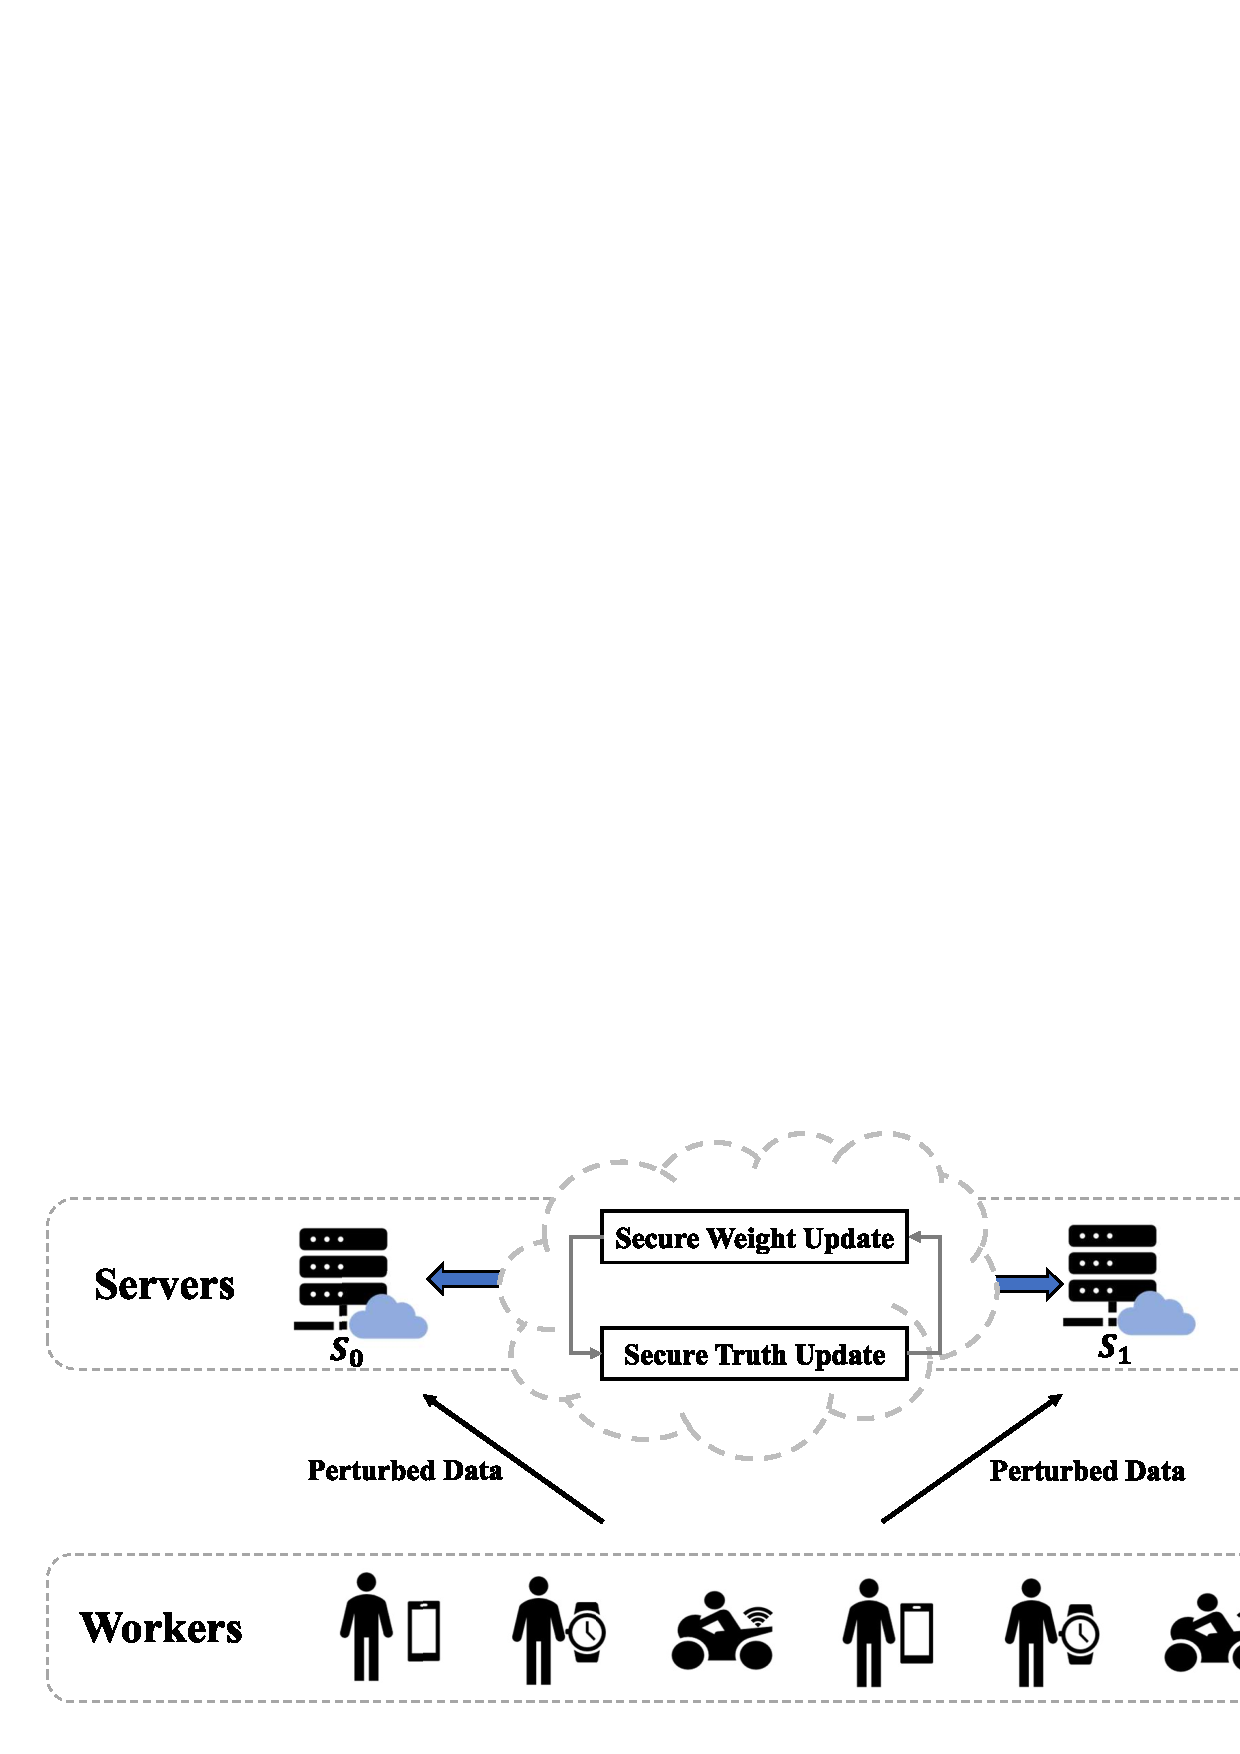
\includegraphics[width=0.96\linewidth]{figures/system_model.pdf}
  \caption{System Model}
  \label{fig:sysmodel}
\end{figure}

\iffalse
\begin{itemize}
  \item \textbf{Workers:} Workers refers to the mobile devices in mobile crowdsensing systems. They are responsible for collecting sensory data of different sensing objects and upload these sensory data to servers. Since most mobile devices are resource-limited, it is not necessary for each worker to collect sensory data of all sensing objects.
  \item \textbf{Servers:} Servers are responsible for analyzing the sensory data for sensing objects. More specifically, after receiving the sensory data uploaded by workers, servers start to estimate the truth for each sensing object. In general, we assume that the servers have sufficient computation and storage capabilities. 
  These two servers are denoted by $S_0$ and $S_1$, respectively.
  % and we use $S_0$ and $S_1$ to denote these two servers respectively.
  % Since our proposed scheme is under two-server setting, 
  % we use $S_0$ and $S_1$ to denote these two servers respectively.
\end{itemize}
\fi

Assume that there are $M$ objects to be sensed, and the number of workers is $K$.
We denote $x_m^k$ as the sensory data of object $m$ provided by worker $k$.
Due to the sparsity of sensory data $\{x_m^k\}_{m=1}^M$, we use an indicator vector $[\phi_1^k, \ldots, \phi_M^k]$ to mark the missing sensory objects where $\phi_m^k = 1$ means worker $k$ has collected the sensory data of object $m$, and $\phi_m^k = 0$ otherwise.
% Since the sensory data $\{x_m^k\}_{m=1}^M$ provided by worker $k$ may be sparse, we use an indicator vector $[\phi_1^k, \ldots, \phi_M^k]$ to mark the missing sensory objects in which $\phi_m^k = 1$ means worker $k$ has collected the sensory data of object $m$, and $\phi_m^k = 0$ otherwise.
% Moreover, worker $k$ also maintains an indicator vector $[\phi_1^k, \ldots, \phi_M^k]$ to mark the missing sensory objects in which $\phi_m^k = 1$ means worker $k$ has collected the sensory data of object $m$, and $\phi_m^k = 0$ otherwise.
Note that if $\phi_m^k = 0$, then the corresponding $x_m^k = 0$.
Besides, we use $w_k$ and $x_m^*$ to denote the weight for worker $k$ and the estimated truth for object $m$, receptively.
% Each worker uploads the sensory data and indicator vector to servers.
% After that, two cloud servers $S_0$ and $S_1$ start to update each worker's weight (denoted by $w_k$ for worker $k$) and then update the estimated truth for each object (denoted by $x_m^*$ for object $m$) iteratively. 

\subsection{Design Goals}
The main goal of our proposed scheme is to design a privacy-preserving truth discovery scheme in the situation where sensory data are sparse.
% First, we need to identify the privacy requirements in the sparse data situation.
Inspired by~\cite{wang_sparse_2020}, the privacy of indicator vector for each worker also needs to be considered for sparse data.
% According to research~\cite{wang_sparse_2020}, the information of which objects are uploaded by a worker may disclose this worker's location trajectory in sparse mobile crowdsensing.
% In other words, the privacy of indicator vector for each worker also needs to be preserved.
Therefore, the main goal is to protect workers' privacy including sensory data, indicator vector, and weights simultaneously.
Besides, considering that most workers are resource-limited, it is also necessary to reduce the computation overhead and communication overhead on the workers' side.

Note that the lazy workers are not involved, because this issue can be solved by integrating incentive mechanism~\cite{xue_inpptd_2020}.
In addition, the issues of inferring missing data from historical data records are challenging and not considered in this work.
% not consider them in this work.

\subsection{Threat Model}~\label{sub:threat}
In the proposed scheme, we assume that all entities are semi-honest, which means that both workers and servers will honestly execute the protocols, but they will also try to infer private information about participants.
For each participant in this system, we assume that there always exist secure channels among workers, $S_0$, and $S_1$.
% As for the communication channels between workers and servers, and 
Besides, similar to other two-sever-based schemes~\cite{miao_lightweight_2017,zhang_reliable_2019}, the two servers are assumed not to collude with each other in this system.
% which is a common assumption in most two-server models~\cite{zhang_lptd_2019,zhang_reliable_2019}.

 % the two servers in our scheme are non-colluding, which is a common assumption in most two-server models~\cite{zhang_lptd_2019,zhang_reliable_2019}.
% Note that the lazy workers are not involved, because this issue can be solved by integrating incentive mechanism~\cite{xue_inpptd_2020}.
% In addition, the issues of inferring missing data from historical data records are challenging and we do not consider them in this work.
% Due to the fact that truth discovery algorithm only considers estimating ground truth from existing sensory data, the issues of inferring missing data are out of the scope of this paper.
 % and we do not consider them in this work.
 % SSL 通道
 % 浮点数处理

\section{Preliminaries}\label{sec4}
% In this section, we introduce the truth discovery algorithm CATD~\cite{li_confidence-aware_2014} and additively homomorphic cryptosystem.
\subsection{CATD}
In general, the truth discovery algorithm CATD~\cite{li_confidence-aware_2014} consists of two parts: weight update and truth update.

\textit{1) Weight Update:} Given the truthful information $\{x_m^*\}_{m=1}^M$, the weight for each worker $k$ is computed as
\begin{equation*}
w_k = \frac{\chi^2_{(1-\alpha/2,\sum_{m=1}^M \phi_m^k)}}{\sum\limits_{m=1}^M \phi_m^k(x_m^k - x_m^*)^2}.
\end{equation*}
Note that $\chi^2$ denotes the Chi-squared distribution, and the system-wide constant $\alpha$ is known as the significance level which is usually a small number such as 0.05.

\textit{2) Truth Update:} Given the weight $w_k$ for each worker $k$, the truth for each object $m$ is computed as
\begin{equation*}
x_m^* = \sum\limits_{k=1}^K w_k x_m^k / \sum\limits_{k=1}^K \phi_m^k w_k.
% x_m^* = \frac{\sum\limits_{k=1}^K w_k x_m^k}{\sum\limits_{k=1}^K \phi_m^k w_k }.
\end{equation*}

In real practice, weight update and truth update should be executed iteratively to achieve more accurate results until the convergence criteria are met.

\subsection{Additively Homomorphic Cryptosystem}\label{sec4-b}
Let $\mathcal{M}$ denote the message space, $\mathcal{C}$ denote the ciphertext space, an additive homomorphic cryptosystem consists of the following four probabilistic poly-time algorithms.

\begin{itemize}
  \item $\mathsf{Setup}(1^\kappa)\to pp$: Taken the input of security parameter $\kappa$, the algorithm returns the public parameter $pp$. Unless otherwise stated, $pp$ is implicitly fed in the following algorithms.
  \item $\mathsf{KeyGen}(1^\kappa)\to (pk, sk)$: Taken the input of security parameter $\kappa$, the algorithm returns the public key $pk$ and private key $sk$.
  \item $\mathsf{Enc}_{pk}(m)\to c$: Given the message $m\in\mathcal{M}$, the encryption algorithm outputs $c$ which is the ciphertext of message $m$.
  \item $\mathsf{Dec}_{sk}(c)\to m$: Given the ciphertext $c$, the decryption algorithm outputs the corresponding plaintext $m$.
\end{itemize}

We claim that the above public-key cryptosystem is additively homomorphic if it satisfies the following properties for some operators $\oplus$ and $\otimes$ in probabilistic polynomial time.

\begin{itemize}
  \item $\forall m_1,m_2\in\mathcal{M}$, given two ciphertexts $c_1 = \mathsf{Enc}_{pk}(m_1)$ and $c_2 = \mathsf{Enc}_{pk}(m_2)$, it holds that $\mathsf{Dec}_{sk}(c_1 \oplus c_2) = m_1 + m_2$.
  \item $\forall m\in\mathcal{M}$, given a constant $a$ and a ciphertext $c=\mathsf{Enc}_{pk}(m)$, it holds that $\mathsf{Dec}_{sk}(a \otimes c) = a \times m$.
\end{itemize}

\subsection{Additive Secret Sharing}
Secret sharing is one of the most important tools in secure multi-party computation.
The additive secret sharing means that a secret $x$ can be randomly split into $n$ shares, for example $x = x_0 + x_1 + \ldots, x_{n-1}$.
The only approach to recover the secret is to collect all $n$ shares.
% To recover the secret, the only way is to 
% The additive secret sharing can be seen as an $(n,n)$-threshold secret sharing 
In this paper, we just pay attention to the situation where $n=2$.
That is, the data owner can randomly split a secret data $x$ into two additive shares $x_0$ and $x_1$, namely, $x = x_0 + x_1$.
For each server $S_i$ $(i\in\{0,1\})$ owns the share $x_i$, the secret $x$ cannot be recovered without the help of $S_{1-i}$.
% the other share of $S_{1-i}$.
In the rest of the paper, we use a share to represent an additive share for simplicity.

\iffalse
\subsection{ABY2.0}
ABY2.0 is an efficient mixed-protocol framework which allows two parties to jointly evaluate a function based on their private inputs~\cite{patra_aby20_2020}.
In this paper, we make use of arithmetic sharing and multiplication protocol of ABY2.0 as the building blocks.
Specificly, we use $\{S_0, S_1\}$ to denote the two parties, and all protocols are executed over an $\ell$-bit ring denoted by $\mathbb{Z}_{2^\ell}$.
For a value $v\in\mathbb{Z}_{2^\ell}$, there are two sharing semantics in ABY2.0, as denoted by $[\cdot]$-sharing and $\langle \cdot \rangle$-sharing as follows.

\textit{$[\cdot]$-sharing:} A value $v\in\mathbb{Z}_{2^\ell}$ is said to be $[\cdot]$-sharing among $\{S_0, S_1\}$, which means the party $S_i$ for $i\in\{0,1\}$ holds $[v]_i$ such that $v = [v]_0 + [v]_1$.

\textit{$\langle \cdot \rangle$-sharing:} A value $v\in\mathbb{Z}_{2^\ell}$ is said to be $\langle \cdot \rangle$-sharing among $\{S_0, S_1\}$, which means the party $S_i$ for $i\in\{0,1\}$ holds $\langle v \rangle_i = (\Delta_v, [\delta_v]_i)$, where $\Delta_v = v + \delta_v$.

It is clear that both $[\cdot]$-sharing and $\langle \cdot \rangle$-sharing supoort linear operations.
For example, given the $\langle \cdot \rangle$-sharing of $a,b$ and public constants $c_1,c_2$, $S_i$ can locally compute $\langle y_i \rangle = c_1 \cdot \langle a \rangle_i + c_2 \cdot \langle b \rangle_i$.
But the multiplication protocol is non-trivial, we give a brief describtion at a high level.
For more detail, please refer to~\cite{patra_aby20_2020}.

The multiplication protocol enables two parties to generate $\langle y \rangle$ where $y = ab$ when given the $\langle \cdot \rangle$-sharing of $a,b$.
\fi

\section{The Proposed Scheme}\label{sec5}
\subsection{Overview}
As we mentioned above, our privacy-preserving truth discovery scheme is designed for scenarios where the sensory data provided by workers are sparse.
In the proposed scheme, workers need to upload indicator vectors to mark which objects they observed.
To satisfy the privacy requirements, it is necessary to protect the privacy of indicator vectors, sensory data, and workers' weights in the same time.
% Although applying GC is a straightforward method to achieve strong privacy preservation, the generation of GC is still a cumbersome task.

% We adopt the additively homomorphic cryptosystem and additive secret sharing in the proposed scheme.
For the sake of illustration, we choose a widely used additively homomorphic cryptosystem called the Paillier cryptosystem~\cite{paillier_public-key_1999} to formulate the homomorphic operations.
 % in the proposed scheme.
In brief, $\forall m_1, m_2, m\in\mathcal{M}$, given the corresponding ciphertexts $c_1,c_2,c$ and a constant $a$, it always holds that 
% $\mathsf{Dec}_{sk}(c_1 \times c_2) = m_1 + m_2, \mathsf{Dec}_{sk}(c_3 ^ a ) = a\times m_3$.
\begin{equation*}
  \begin{split}
  \mathsf{Dec}_{sk}(c_1 \times c_2) = m_1 + m_2, \mathsf{Dec}_{sk}(c ^ a ) = a\times m.
  \end{split}
\end{equation*}
% 浮点数处理

Note that the above Paillier cryptosystem only works over integers, while the sensory data in our scheme may be floating-point numbers.
To handle this situation, a typical approach is to round the floating-point numbers by multiplying a factor $L$, and the final results can be recovered by dividing $L$~\cite{zheng_learning_2018,xue_inpptd_2020}.

To reduce the complicated operations on the workers' side, we shift all heavy cryptographic operations to the servers' side.
In other words, workers only need to generate shares and upload them to two servers respectively.
% split data into two parts randomly and then upload them to two servers respectively.
After that, the truths can be estimated by two servers.
The whole procedure can be divided into 5 phases: {\em Initialization}, {\em Report}, {\em Pre-Processing}, {\em Secure Weight Update} and {\em Secure Truth Update}.

\subsection{Initialization Phase}
% As described in Section~\ref{sec3-A}, assume that there are $K$ participating workers and $M$ sensing objects in the system.
In this phase, $S_0$ first generates an asymmetric key pair $(pk, sk)$ of the additively homomorphic cryptosystem by invoking $\mathsf{KeyGen}(\cdot)$.
% in Section~\ref{sec4-b}.
% Note that if this phase is executed for the first time, the initial ground truths $\{x_m^*\}_{m=1}^M$ are chosen randomly.
Then $S_0$ sets a small number for the significant level $\alpha$ ($\alpha$ is set to 0.05 by default) and randomly generates the initial truths $\{x_m^*\}_{m=1}^M$.
Finally, $S_0$ publishes the public key $pk$ along with the significant level $\alpha$, and sends the initial truths to $S_1$.

\subsection{Report Phase}
In this phase, each worker collects sensory data for distinct objects.
Taking worker $k$ as an example, after obtaining a set of sensory data $\{x_m^k\}_{m=1}^M$ and generating an indicator vector $\{\phi_m^k\}_{m=1}^M$, worker $k$ computes $y_k = \chi^2_{(1-\alpha/2, \sum_{m=1}^M \phi_m^k)}$.
Then for each object $m$, worker $k$ computes $\tilde{\phi}_m^k = \phi_m^k / y_k$.
After that, worker $k$ computes the shares of $x_m^k$, $\phi_m^k$ and $\tilde{\phi}_m^k$.
Namely, $x_m^k = x_{m,0}^k + x_{m,1}^k$, $\phi_m^k = \phi_{m,0}^k + \phi_{m,1}^k$, $\tilde{\phi}_m^k = \tilde{\phi}_{m,0}^k + \tilde{\phi}_{m,1}^k$.
Finally worker $k$ uploads $\{x_{m,0}^k, \phi_{m,0}^k ,\tilde{\phi}_{m,0}^k\}_{m=1}^M$ to $S_0$, $\{x_{m,1}^k, \phi_{m,1}^k, \tilde{\phi}_{m,1}^k\}_{m=1}^M$ to $S_1$.
 % splits $x_m^k$, $\phi_m^k$ and $\tilde{\phi}_m^k$ into two parts randomly (i.e., $x_m^k = x_{m,0}^k + x_{m,1}^k$, $\phi_m^k = \phi_{m,0}^k + \phi_{m,1}^k$, $\tilde{\phi}_m^k = \tilde{\phi}_{m,0}^k + \tilde{\phi}_{m,1}^k$, where $\{x_{m,0}^k, \phi_{m,0}^k, \tilde{\phi}_m^k\}_{m=1}^M$ are chosen randomly), and uploads $\{x_{m,0}^k, \phi_{m,0}^k ,\tilde{\phi}_{m,0}^k\}_{m=1}^M$ to $S_0$, $\{x_{m,1}^k, \phi_{m,1}^k, \tilde{\phi}_{m,1}^k\}_{m=1}^M$ to $S_1$.
When the uploading process is complete, worker $k$ can go offline.

\subsection{Pre-Processing Phase}
We emphasize that this phase is executed by $S_0$.
For worker $k$, $S_0$ first computes $C_0^k$ as: 
\begin{equation*}
  \begin{split}
  C_0^k = \mathsf{Enc}_{pk}\left[\sum_{m=1}^M \tilde{\phi}_{m,0}^k \left(x_{m,0}^k\right)^2\right].
  \end{split}
\end{equation*}
Then $S_0$ encrypts $\{x_{m,0}^k, (x_{m,0}^k)^2, \tilde{\phi}_{m,0}^k,\tilde{\phi}_{m,0}^k\cdot x_{m,0}^k\}_{m,k=1}^{M,K}$ respectively.
These ciphertexts are typically denoted by $C_{pack1}$.
Finally, $S_0$ sends $\{C_0^k\}_{k=1}^K$ and $C_{pack1}$ to $S_1$.

\subsection{Secure Weight Update Phase}
% The iteration phase consists of the secure weight update phase and secure truth update phase.
In this phase, upon receiving the ciphertexts, $S_1$ computes $C_1^k$,$C_2^k$,$C_3^k$,$C_4^k$ as follows.
\begin{equation*}
  % \begin{split}
  \left\{\begin{aligned}
    C_1^k & = \prod_{m=1}^M\left[ \mathsf{Enc}_{pk}{\left[\left(x_{m,0}^k\right)^2\right]}^{\tilde{\phi}_{m,1}^k} \right] , \\
    C_2^k & =  \prod_{m=1}^M\left[ \left[\mathsf{Enc}_{pk}\left(x_{m,0}^k\right)\right]^{2\left(x_{m,1}^k - x_m^*\right)\tilde{\phi}_{m,1}^k}\right] \times \\
          & \qquad \prod_{m=1}^M\left[ \left[\mathsf{Enc}_{pk}\left(\tilde{\phi}_{m,0}^k x_{m,0}^k\right)\right]^{2\left(x_{m,1}^k - x_m^*\right)} \right] , \\
     C_3^k & = \prod_{m=1}^M\left[ \mathsf{Enc}_{pk}\left(\tilde{\phi}_{m,0}^k\right)^{\left(x_{m,1}^k - x_m^*\right)^2} \right] , \\
     C_4^k & = \mathsf{Enc}_{pk}\left[\sum_{m=1}^M \tilde{\phi}_{m,1}^k \left(x_{m,1}^k - x_m^*\right)^2\right] .
    \end{aligned}
    \right.
  % \end{split}
\end{equation*}

\iffalse
\begin{equation*}
  \begin{split}
  C_1^k & = \prod_{m=1}^M\left[ \mathsf{Enc}_{pk}{\left[\left(x_{m,0}^k\right)^2\right]}^{\tilde{\phi}_{m,1}^k} \right] \\
  % & = \mathsf{Enc}_{pk}\left[ \sum_{m=1}^M \tilde{\phi}_{m,1}^k \left(x_{m,0}^k\right)^2\right]
  \end{split}
\end{equation*}
\begin{equation*}
  \begin{split}
  C_2^k & =  \prod_{m=1}^M\left[ \left[\mathsf{Enc}_{pk}\left(x_{m,0}^k\right)\right]^{2\left(x_{m,1}^k - x_m^*\right)\tilde{\phi}_{m,1}^k}\right] \cdot \\
          & \qquad \prod_{m=1}^M\left[ \left[\mathsf{Enc}_{pk}\left(\tilde{\phi}_{m,0}^k x_{m,0}^k\right)\right]^{2\left(x_{m,1}^k - x_m^*\right)} \right] \\
          % & = \mathsf{Enc}_{pk}\left[\sum_{m=1}^M 2\tilde{\phi}_m^k x_{m,0}^k\left(x_{m,1}^k - x_m^*\right)\right]  \\
  \end{split}
\end{equation*}
\begin{equation*}
  \begin{split}
    C_3^k & = \prod_{m=1}^M\left[ \mathsf{Enc}_{pk}\left(\tilde{\phi}_{m,0}^k\right)^{\left(x_{m,1}^k - x_m^*\right)^2} \right] \\
    % & = \mathsf{Enc}_{pk}\left[\sum_{m=1}^M \tilde{\phi}_{m,0}^k\left(x_{m,1}^k - x_m^*\right)^2\right] \\
  \end{split}
\end{equation*}
\begin{equation*}
  \begin{split}
    C_4^k & = \mathsf{Enc}_{pk}\left[\sum_{m=1}^M \tilde{\phi}_{m,1}^k \left(x_{m,1}^k - x_m^*\right)^2\right]
  \end{split}
\end{equation*}
\fi

To preserve the privacy of workers' weights, $S_1$ chooses a random value $b_k$ and computes the ciphertexts $C_k$ as 
\begin{equation*}
  \begin{split}
    C_k = & \left(C_0^k\cdot C_1^k\cdot C_2^k\cdot C_3^k \cdot C_4^k\right)^{b_k} .\\
  \end{split}
\end{equation*}
Finally $S_1$ sends $\{C_k\}_{k=1}^K$ to $S_0$.
% Note that if this phase is executed for the first time, the initial ground truths $\{x_m^*\}_{m=1}^M$ are chosen randomly.
After receiving $\{C_k\}_{k=1}^K$, $S_0$ decrypts $C_k$ with its private key and obtains the perturbed weight $\tilde{w}_k$ of worker $k$ as follows,
\begin{equation}
  \begin{split}
    \tilde{w}_k = \frac{1}{\mathsf{Dec}_{sk}\left(C_k\right)} = \frac{w_k}{b_k}.
  ~\label{eq:wk}
  \end{split}
\end{equation}

\subsection{Secure Truth Update Phase}
In the truth update phase, $S_0$ first encrypts $\{\tilde{w}_k\}_{k=1}^K$ and $\{\tilde{w}_k\cdot x_{m,0}^k, \tilde{w}_k\cdot \phi_{m,0}^k\}_{m,k=1}^{M,K}$ respectively.
The sets of ciphertexts are denoted by $C_{pack2}$.
Finally $S_0$ sends $C_{pack2}$ to $S_1$.

After receiving the ciphertexts, $S_1$ computes $C_5^m$ and $C_6^m$ as follows,
\begin{equation*}
  \begin{split}
    C_5^m & = \prod_{k=1}^K\left[\left[\mathsf{Enc}_{pk}\left(\tilde{w}_k\cdot x_{m,0}^k\right)\cdot \left[\mathsf{Enc}_{pk}\left(\tilde{w}_k\right)\right]^{x_{m,1}^k}\right]^{b_k} \right] \\
    & = \mathsf{Enc}_{pk}\left[\sum_{k=1}^K w_kx_m^k\right] , \\
  \end{split}
\end{equation*}
\begin{equation*}
  \begin{split}
    C_6^m & = \prod_{k=1}^K \left[ \left[ \mathsf{Enc}_{pk}(\tilde{w}_k\cdot \phi_{m,0}^k) \cdot \left[\mathsf{Enc}_{pk}(\tilde{w}_k)\right]^{\phi_{m,1}^k}\right]^{b_k} \right] \\
     & = \mathsf{Enc}_{pk}\left[\sum_{k=1}^K w_k\phi_m^k \right] . \\
  \end{split}
\end{equation*}
Finally, $S_1$ sends $\{C_5^m\}_{m=1}^M$ and $\{C_6^m\}_{m=1}^M$ to $S_0$.
Then $S_0$ decrypts these ciphertexts and obtains the estimated truth as follows,
\begin{equation}
  \begin{split}
    x_m^* = \frac{\mathsf{Dec}_{sk}(C_5^m)}{\mathsf{Dec}_{sk}(C_6^m)} = \sum\limits_{k=1}^K w_kx_m^k / \sum\limits_{k=1}^K w_k\phi_m^k .
    % x_m^* = \frac{\mathsf{Dec}_{sk}(C_5^m)}{\mathsf{Dec}_{sk}(C_6^m)} = \frac{\sum\limits_{k=1}^K w_kx_m^k}{\sum\limits_{k=1}^K w_k\phi_m^k} .
  \end{split}
  \label{eq:xm}
\end{equation}

\section{System Analysis}\label{sec6}
% \subsection{Security Analysis}
\subsection{Correctness}
Since the correctness of decryption can be guaranteed by the additively homomorphic cryptosystem, we only need to prove that the Eq.~\ref{eq:wk} and Eq.~\ref{eq:xm} hold.
% To prove the correctness of the proposed scheme, 
The correctness of Eq.~\ref{eq:xm} is straightforward, here we give the correctness analysis of Eq.~\ref{eq:wk}.
According to the properties of the additively homomorphic cryptosystem, we have
\begin{equation*}
  \begin{split}
  C_0^k C_1^k & = \mathsf{Enc}_{pk}\left[\sum_{m=1}^M \tilde{\phi}_{m,0}^k\left(x_{m,0}^k\right)^2 + \tilde{\phi}_{m,1}^k\left(x_{m,0}^k\right)^2  \right] \\
   & = \mathsf{Enc}_{pk}\left[\sum_{m=1}^M \tilde{\phi}_m^k\left(x_{m,0}^k\right)^2 \right] , \\
  \end{split}
\end{equation*}
\begin{equation*}
  \begin{split}
  C_3^kC_4^k & = \mathsf{Enc}_{pk}\left[\sum_{m=1}^M \left(\tilde{\phi}_{m,0}^k + \tilde{\phi}_{m,1}^k\right) \left(x_{m,1}^k-x_m^*\right)^2 \right] \\
  & = \mathsf{Enc}_{pk}\left[\sum_{m=1}^M \tilde{\phi}_m^k\left(x_{m,1}^k - x_m^*\right)^2\right] . \\
  \end{split}
\end{equation*}
Since $\tilde{\phi}_m^k (x_{m,0}^k)^2 + 2\tilde{\phi}_m^kx_{m,0}^k\left(x_{m,1}^k - x_m^*\right) + \tilde{\phi}_m^k(x_{m,1}^k - x_m^*)^2 = \tilde{\phi}_m^k (x_{m,0}^k + x_{m,1}^k - x_m^*)^2$, then we can further obtain
\begin{equation*}
  \begin{split}
  C_k & = \left(C_0^k \cdot C_1^k\cdot C_2^k \cdot C_3^k \cdot C_4^k\right)^{b_k} \\
   & = \left[\mathsf{Enc}_{pk}\left[\sum_{m=1}^M \tilde{\phi}_m^k (x_{m,0} + x_{m,1} - x_m^*)^2 \right]\right]^{b_k} \\
  & = \mathsf{Enc}_{pk}\left[b_k \sum_{m=1}^M \tilde{\phi}_m^k (x_m - x_m^*)^2 \right] . \\
  \end{split}
\end{equation*}
Hence, the perturbed weight $\tilde{w}_k$ can be written as
\begin{equation*}
  \begin{split}
  \tilde{w}_k & = \frac{1}{\mathsf{Dec}_{sk}\left(C_k\right)} = \frac{1}{b_k \sum\limits_{m=1}^M \tilde{\phi}_m^k (x_m - x_m^*)^2} = \frac{w_k}{b_k} . \\
  % & = \frac{1}{b_k} \cdot \frac{y_k}{\sum_{m=1}^M \phi_m^k (x_m - x_m^*)^2} \\
  % & = \frac{w_k}{b_k} . \\
  \end{split}
\end{equation*}
Therefore, the correctness of Eq.~\ref{eq:wk} holds.

\iffalse
\begin{table*}[t]
    \centering
    \caption{Communication Overhead}
    \linespread{1.3}\selectfont
    \begin{tabular}{l c c c c c c}
        \hline
        \hline
        \multirow{2}*{Scheme} &  \multicolumn{2}{c}{System Initialization} & \multicolumn{3}{c}{Key Generation and Distribution}& Encryption/Decryption\\
        \cmidrule(lr){2-3}\cmidrule(lr){4-6} \cmidrule{7-7} & CA & AA & CA &AA &User & Owner\\
        \hline
        Li & Not exist & N/A  & Not exist & $3N_{i,j}\|p\|$ & $3N_{i,j}\|p\|$ & $(3+2N_{a,2})\|p\|$ \\
        Chase & $N_A\|p\|+N_{a,1}\|p\|$ & $(N_i+1)\|p\|$ & $\|p\|$ & $N_{i,j}\|p\|$ & $(N_{i,j}+1)\|p\|$ & $(2+N_{a,2})\|p\|$ \\
        Chase & Not exist & $(N_A-1)\|p\|$ & Not exist & $(N_{i,j}+5)\|p\|$ & $5(N_A-1)\|p\|+N_{i,j}\|p\|$ & $(2+N_{a,2})\|p\|$ \\     
        \hline
        \hline
    \end{tabular}
\end{table*}
\fi

\subsection{Security Discussion}

Note that our design goal is to protect the privacy of sensory data, indicator vectors and weights for each worker simultaneously.
% In this regard, we present the following theorem.
% \begin{theorem}
%   Suppose that workers, $S_0$ and $S_1$ satisfy the threat model in this paper, the additively homomorphic cryptosystem is secure, then the privacy of workers' sensory data, indicator vectors, and weights can be protected under the proposed scheme.
% \end{theorem}
% {\em Proof.} 
According to the threat model in Section~\ref{sub:threat}, each entity is assumed to be semi-honest, and two servers are non-colluding.
Since workers do not take part in the iteration phase, we only need to consider that the privacy of $x_m^k$, $\phi_m^k$ and $w_k$ are not disclosed from the views of $S_0$ and $S_1$.
 % to $S_0$ or $S_1$ for each worker $k$.

For $S_0$, it only knows $\{x_{m,0}^k, \phi_{m,0}^k, \tilde{\phi}_{m,0}^k\}_{m=1}^M$, $C_k$, $C_5^m$ and $C_6^m$.
$S_0$ can decrypt $C_k$, $C_5^m$, $C_6^m$, and further obtain the perturb weight $\tilde{w}_k$ along with the aggregation information such as $\sum\limits_{k=1}^K w_k x_m^k$ and $\sum\limits_{k=1}^K w_k \phi_m^k$.
Since $x_{m,1}^k$ and $\phi_{m,1}^k$ are generated randomly from additive secret sharing by worker $k$, $b_k$ is chosen randomly by $S_1$.
% Since $x_{m,1}^k$ and $\phi_{m,1}^k$ are generated randomly by worker $k$, $b_k$ is chosen randomly by $S_1$.
Without knowing $x_{m,1}^k$, $\phi_{m,1}^k$ and $b_k$, $S_0$ cannot infer $x_m^k$, $\phi_m^k$ and $w_k$ for worker $k$.

For $S_1$, it only knows $\{x_{m,1}^k, \phi_{m,1}^k, \tilde{\phi}_{m,1}^k\}_{m=1}^M$, $C_0^k$, $C_{pack1}$ and $C_{pack2}$.
Similarly, since $x_{m,0}^k$ and $\phi_{m,0}^k$ are generated randomly from additive secret sharing by worker $k$, $S_1$ cannot infer $x_m^k$ and $\phi_m^k$ for worker $k$ without knowing $x_{m,0}^k$ and $\phi_{m,0}^k$.
Note that $C_0^k$, $C_{pack1}$ and $C_{pack2}$ are ciphertexts under additively homomorphic cryptosystem, $S_1$ has no mechanism to decrypt them without the private key $sk$, and hence cannot learn worker's weight $w_k$ even it knows the ciphertext $C_k$.

\section{Performance Evaluation}\label{sec7}
In this section, we evaluate the performance of the proposed scheme in terms of accuracy, convergence, computation overhead, and communication overhead.
% Specifically, we choose Paillier homomorphic cryptosystem~\cite{paillier_public-key_1999} as the additively homomorphic cryptosystem in our scheme.
All procedures are conducted on a computer with an Intel Core i5-10400 CPU (4.30 GHz) and 16GB RAM running Linux operation system.
We invoke the Python-Paillier library~\cite{PythonPaillier} for rapidly building advance cryptosystems (key size is set to 2048 bits by default).
All experiments are executed 10 times and we take the average results.
For the sake of illustration, we use $\gamma$ to denote the sparsity of sensory data.
$\gamma$ is defined as $\gamma = 1 - (\sum\limits_{m=1}^M\sum\limits_{k=1}^K\phi_m^k) / (M\cdot K)$.
% The sparsity $\gamma$ is fixed as 0.2 by default.
Hereafter, unless otherwise stated, the default sparsity is set to 0.2 by default.
% \begin{equation*}
%   \gamma = 1 - (\sum_{m=1}^M\sum_{k=1}^K\phi_m^k) / (M\cdot K).
% \end{equation*}

\subsection{Accuracy}
Since the CATD framework is adopted as the fundamental truth discovery algorithm in our proposed scheme, we first measure the accuracy of estimated ground truth between our proposed scheme and CATD.
Similar to~\cite{zhang_reliable_2019,xue_inpptd_2020}, we use the Root of Mean Squared Error (RMSE) defined as $(\sum\limits_{m=1}^M (x_m^* - \hat{x}_m)/M)^{\frac{1}{2}}$ to evaluate the deviation between the estimated truths $\{x_m^*\}_{m=1}^M$ and the ground truths $\{\hat{x}_m\}_{m=1}^M$.
In this experiment, the number of objects is fixed as 20, the number of workers varies from 10 to 50.
 % and sparsity of sensory data are fixed as 20 and 0.2 respectively, the number of workers varies from 5 to 25.
As shown in Fig.~\ref{fig:rmse1}, we observe that the proposed scheme achieves a similar accuracy to the baseline algorithm CATD.
Additionally, the estimated truths are closer to the real ground truths with the increase in the number of workers.
\begin{figure}[htbp]
  \centering 
  \subfloat[Accuracy Comparison with CATD]{ 
    \label{fig:rmse1}
    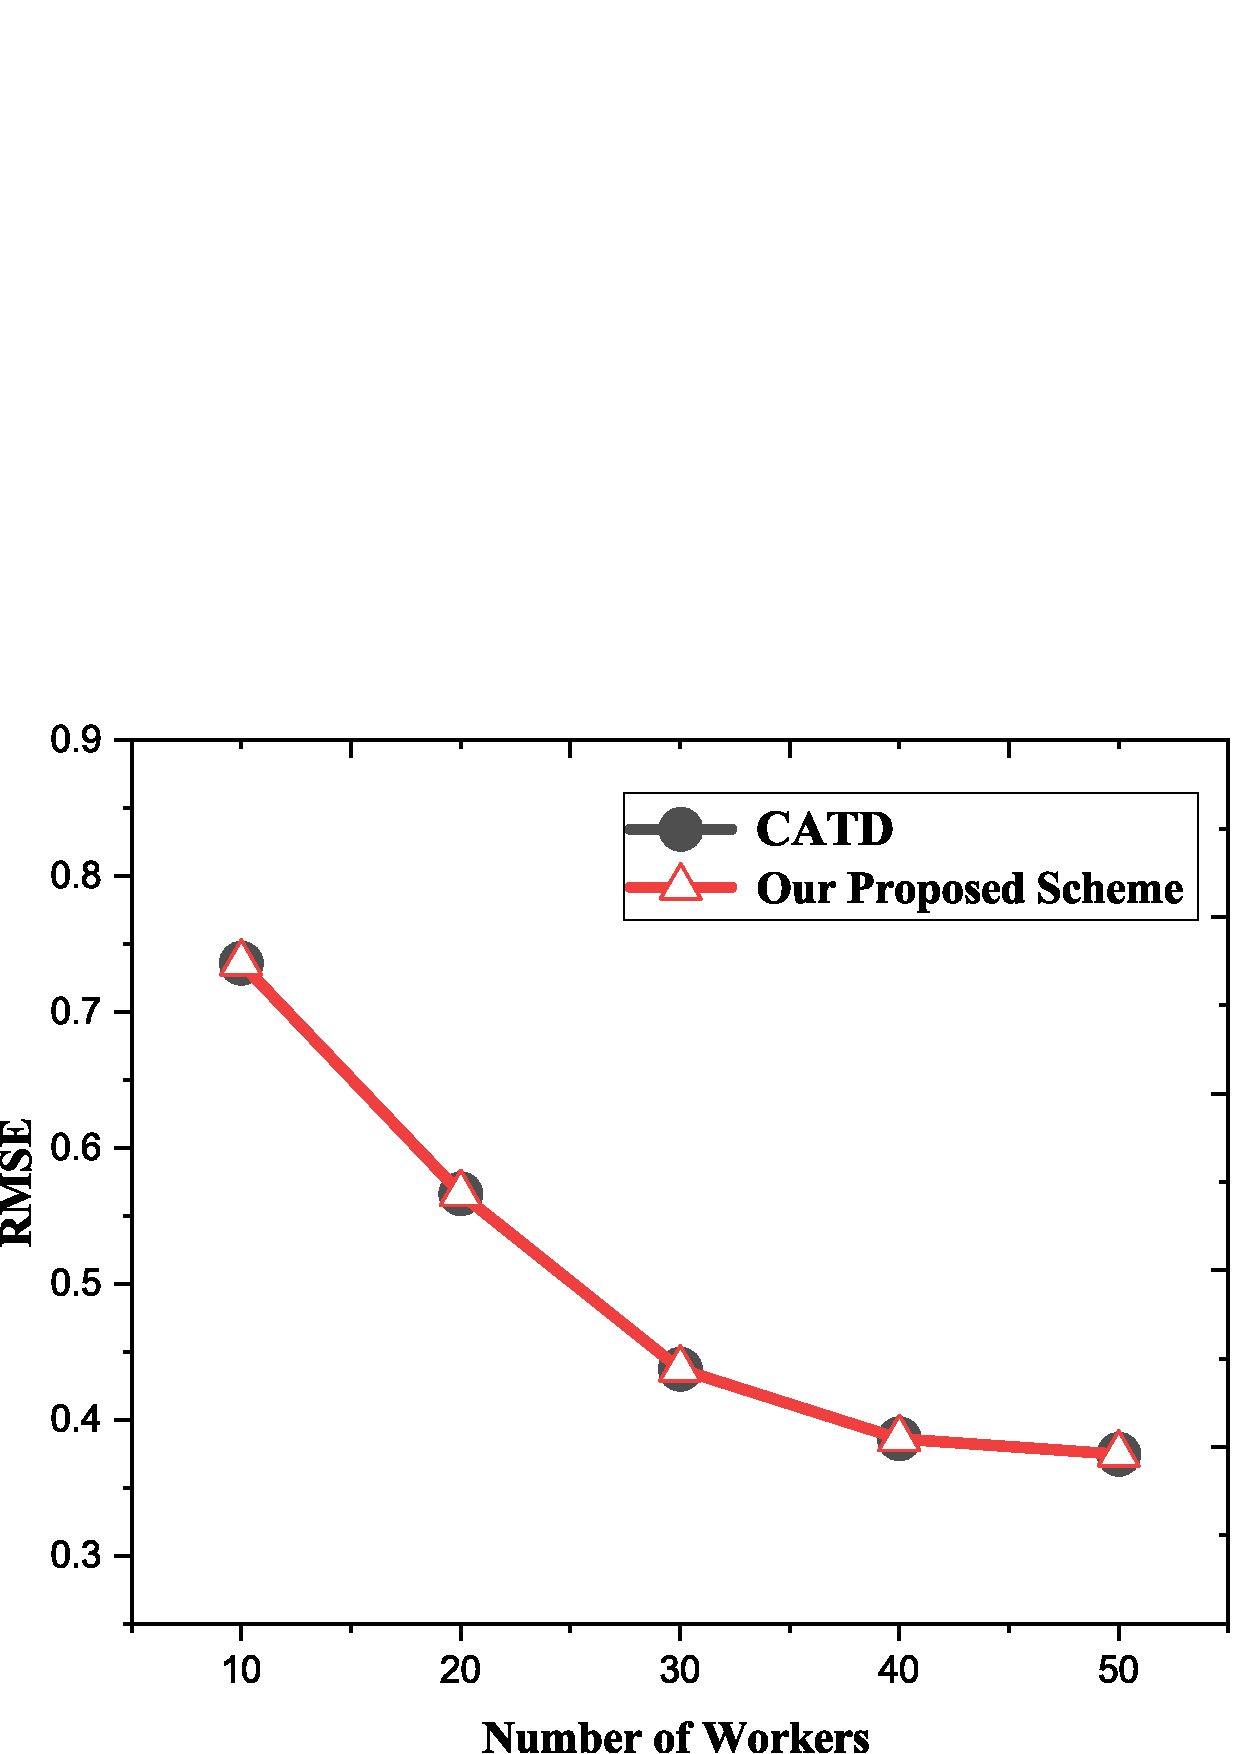
\includegraphics[width=0.5\linewidth]{figures/rmse1.pdf}}
  \subfloat[The Impact of Different Sparsity]{ 
    \label{fig:rmse2} 
    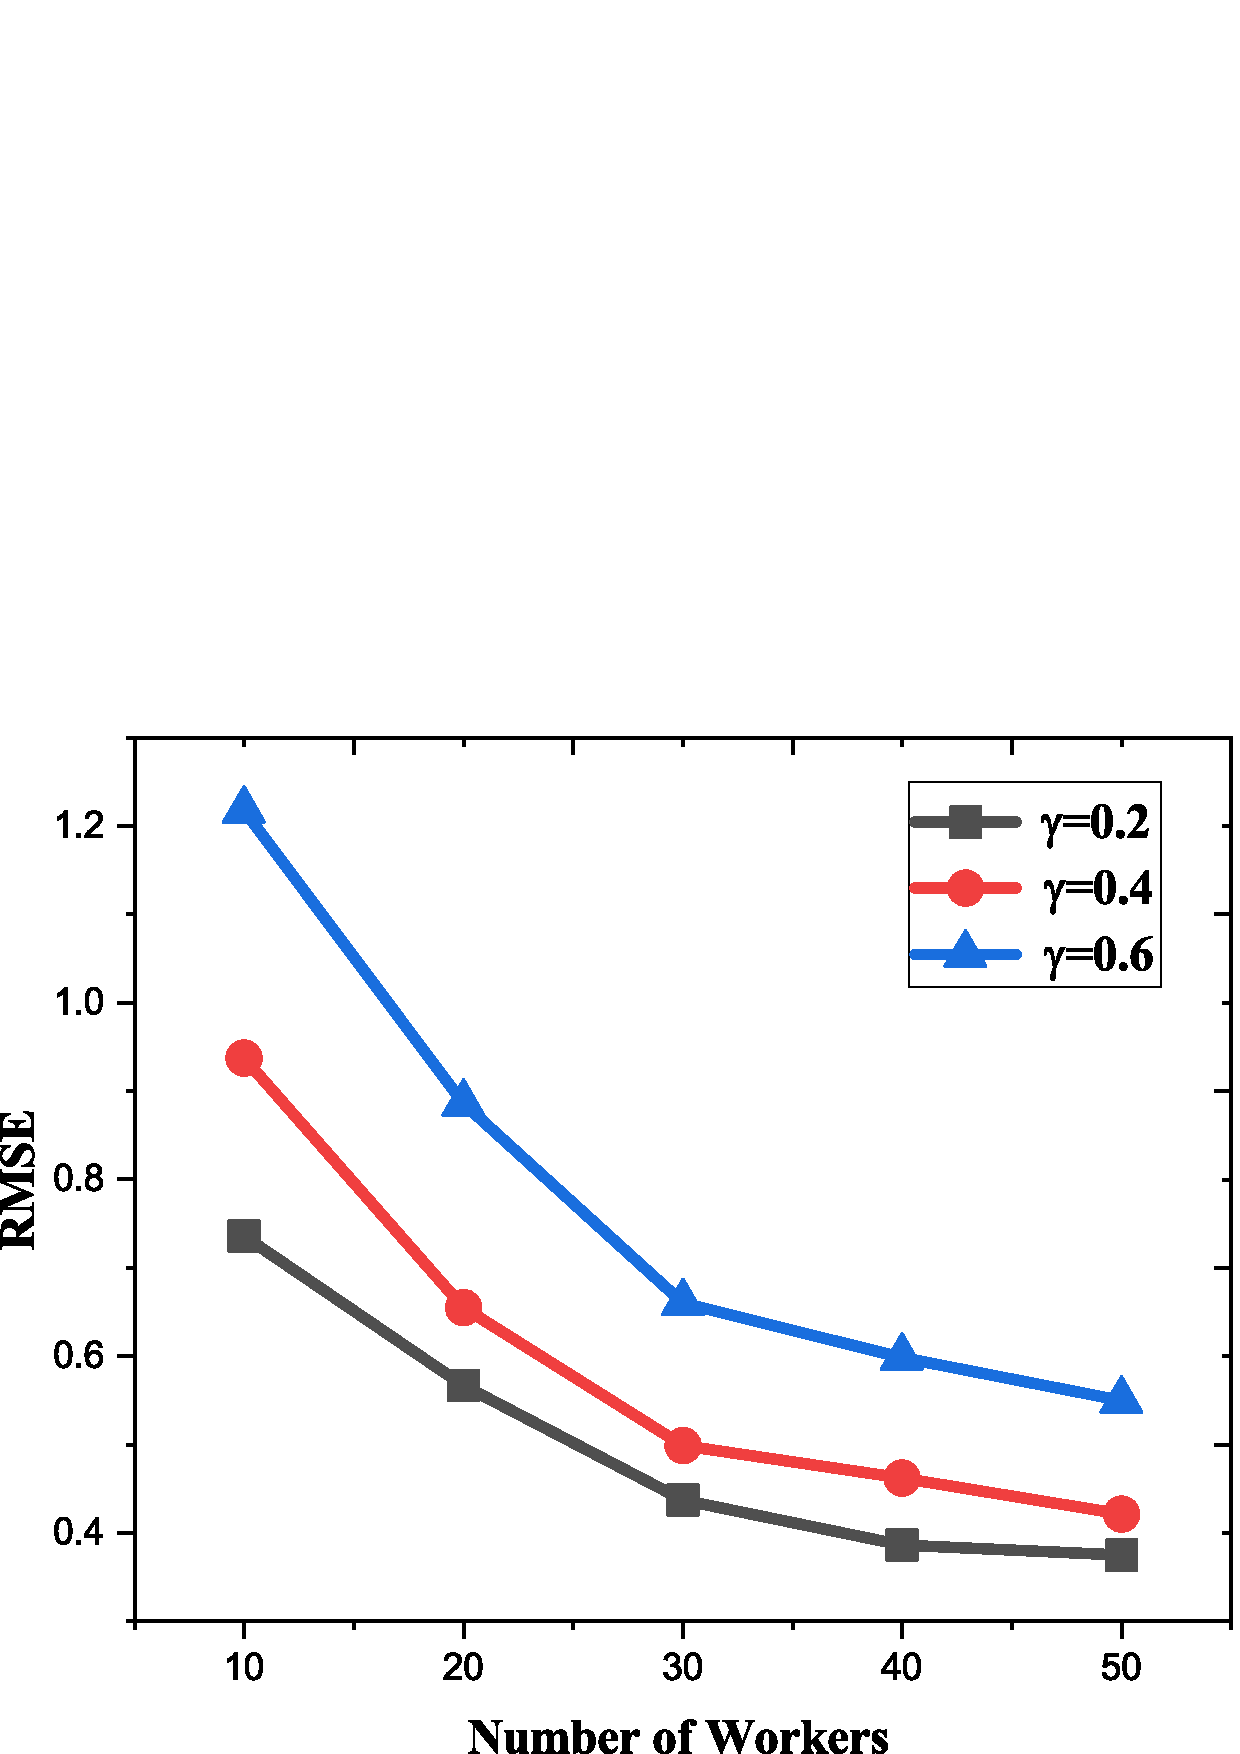
\includegraphics[width=0.5\linewidth]{figures/rmse2.pdf}} 
  \caption{Accuracy Evaluation}
  \label{fig:rmse} 
\end{figure}
To further analyze the impact of sparsity $\gamma$ for accuracy, we conduct the experiment under different sparsity settings from 0.2 to 0.6.
The results in Fig.~\ref{fig:rmse2} show that in a high sparsity situation, it is necessary to recruit more workers to get more accurate results.
% decrease the deviation between estimated truths with real ground truths.

\subsection{Convergence}
As for convergence, we use $\sum\limits_{m=1}^M (x_m^t - x_m^{t-1})^2$ as the convergence value in the $t$-th iteration, where $x_m^t$ is the estimated truth in $t$-th iteration and $x_m^0$ is initialized randomly.
In this experiment, the number of workers and objects are fixed as 10 and 20 respectively.
As illustrated in Fig.~\ref{fig:conver}, the convergence speed is very fast at the first few iterations.
Meanwhile, the sparsity has little impact on the convergence.
\begin{figure}[htbp]
  \centering
  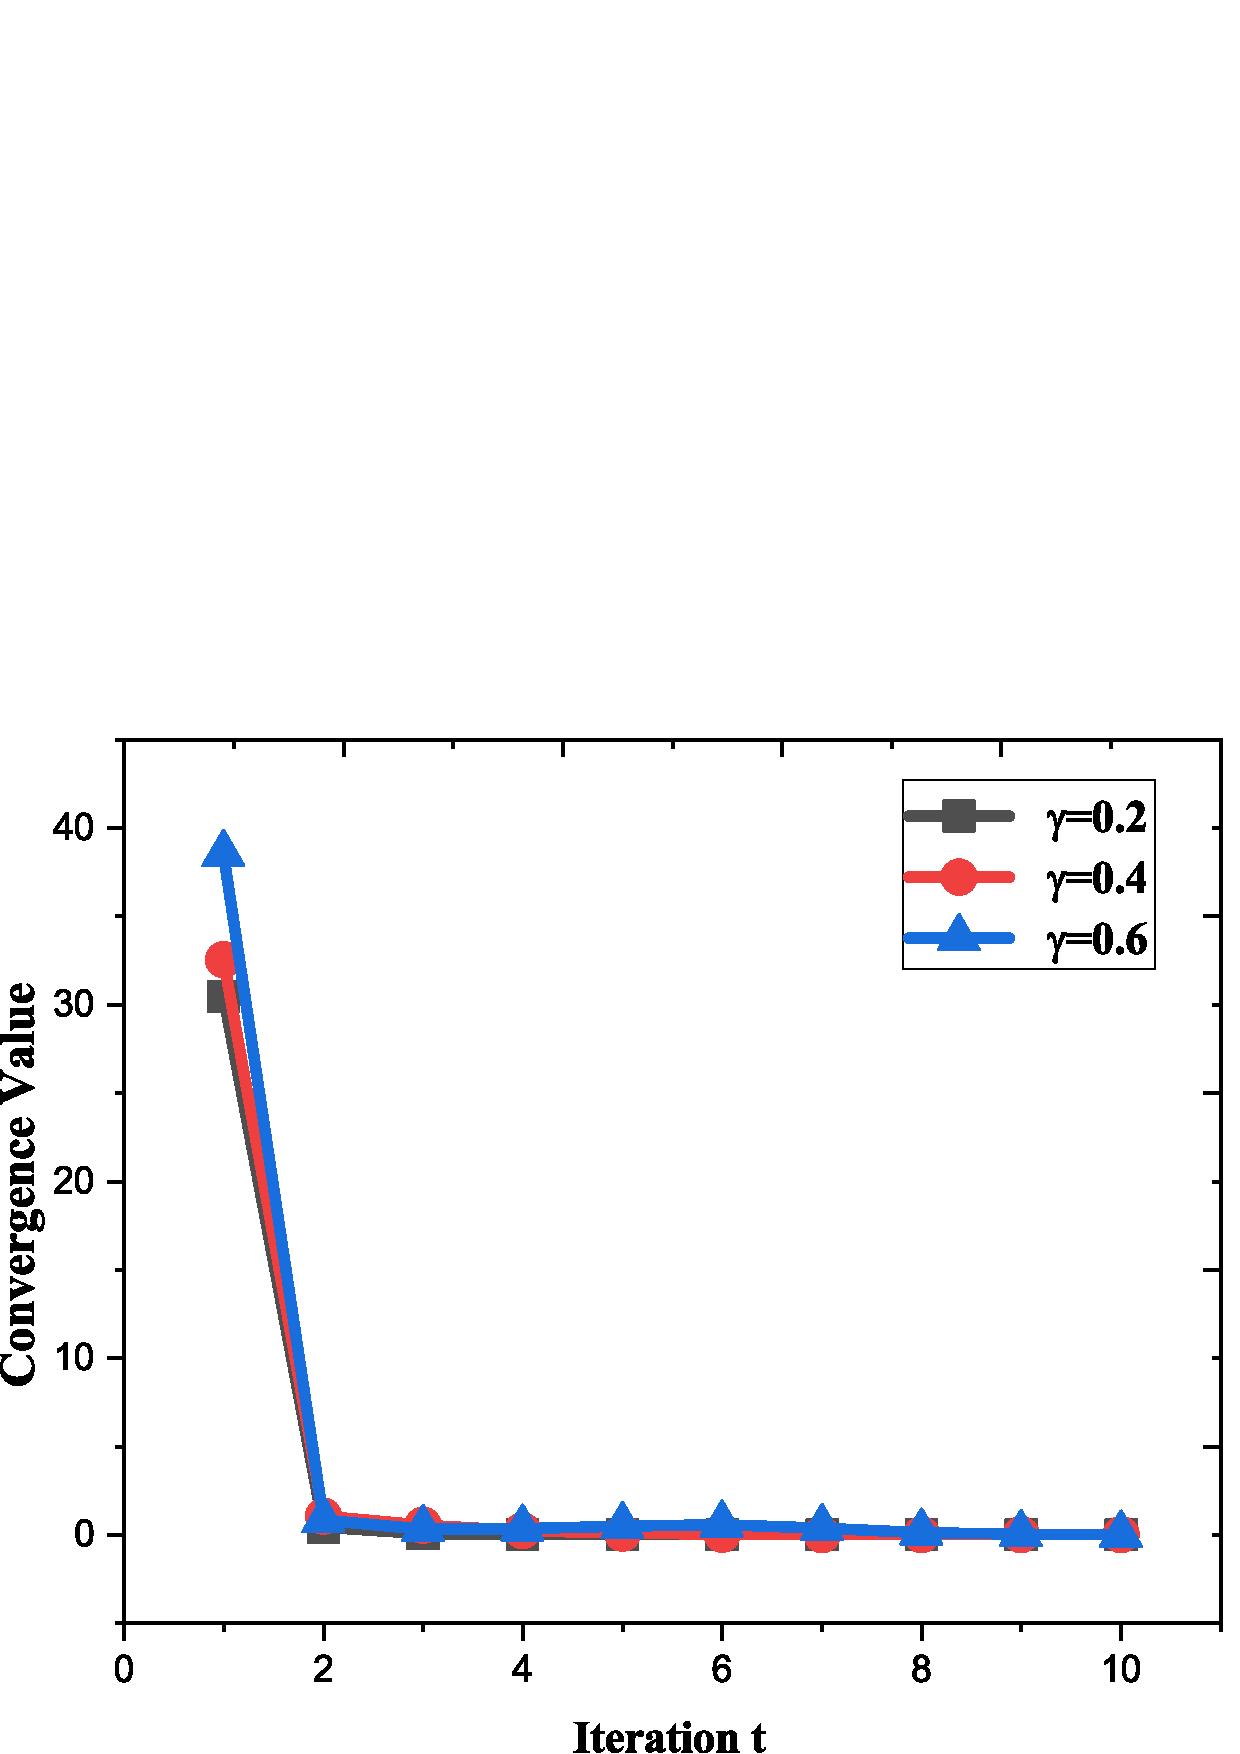
\includegraphics[width=0.60\linewidth]{figures/conver.pdf}
  \caption{Convergence Evaluation}
  \label{fig:conver}
\end{figure}

\subsection{Efficiency Evaluation}
In this part, we measure the performance of computation overhead and communication overhead respectively.
% In this experiment, the sparsity is fixed as 0.2 by default.
% Hereafter, unless otherwise stated, the default sparsity is set to 0.2.
TABLE~\ref{tab:computation} lists the computation overhead of workers and $S_0$ in non-iteration phases including the report phase and pre-processing phase with the different number of objects and workers.
We observe the computation cost of workers is negligible compared to $S_0$ since there are no heavy cryptographic operations on the workers' side.

\begin{table}[htbp]
  \centering
  \caption{Computation Overhead in Non-Iteration Phases (s)}~\label{tab:computation}
  \linespread{1.3}\selectfont
  \begin{adjustbox}{max width=0.46\textwidth}
  \begin{tabular}{l l c c c}
    \hline
    \hline
    \multicolumn{2}{c}{\multirow{2}*{Number of Workers and Objects}} & \multicolumn{1}{c}{Report Phase} & \multicolumn{1}{c}{Pre-Processing Phase} \\
    \cmidrule(lr){3-3}\cmidrule(lr){4-4} & & Workers & $S_0$ \\
    \hline
     \multirow{3}*{$K=10$} & $M=20$ & 0.0011 & 6.93 \\
      & $M=40$ & 0.0011 & 20.98 \\
      & $M=60$ & 0.0012 & 34.86 \\
     \cmidrule(lr){1-2}
     \multirow{3}*{$M=20$} & $K=20$ & 0.0049 & 14.04\\
     & $K=40$ & 0.0059 & 42.41\\
     & $K=60$ & 0.0104 & 70.92 \\
    \hline
    \hline
  \end{tabular}
  \end{adjustbox}
\end{table}

\begin{figure}[!ht]
  \centering 
  \subfloat[$K = 10 $]{ 
    \label{fig:comp1}
    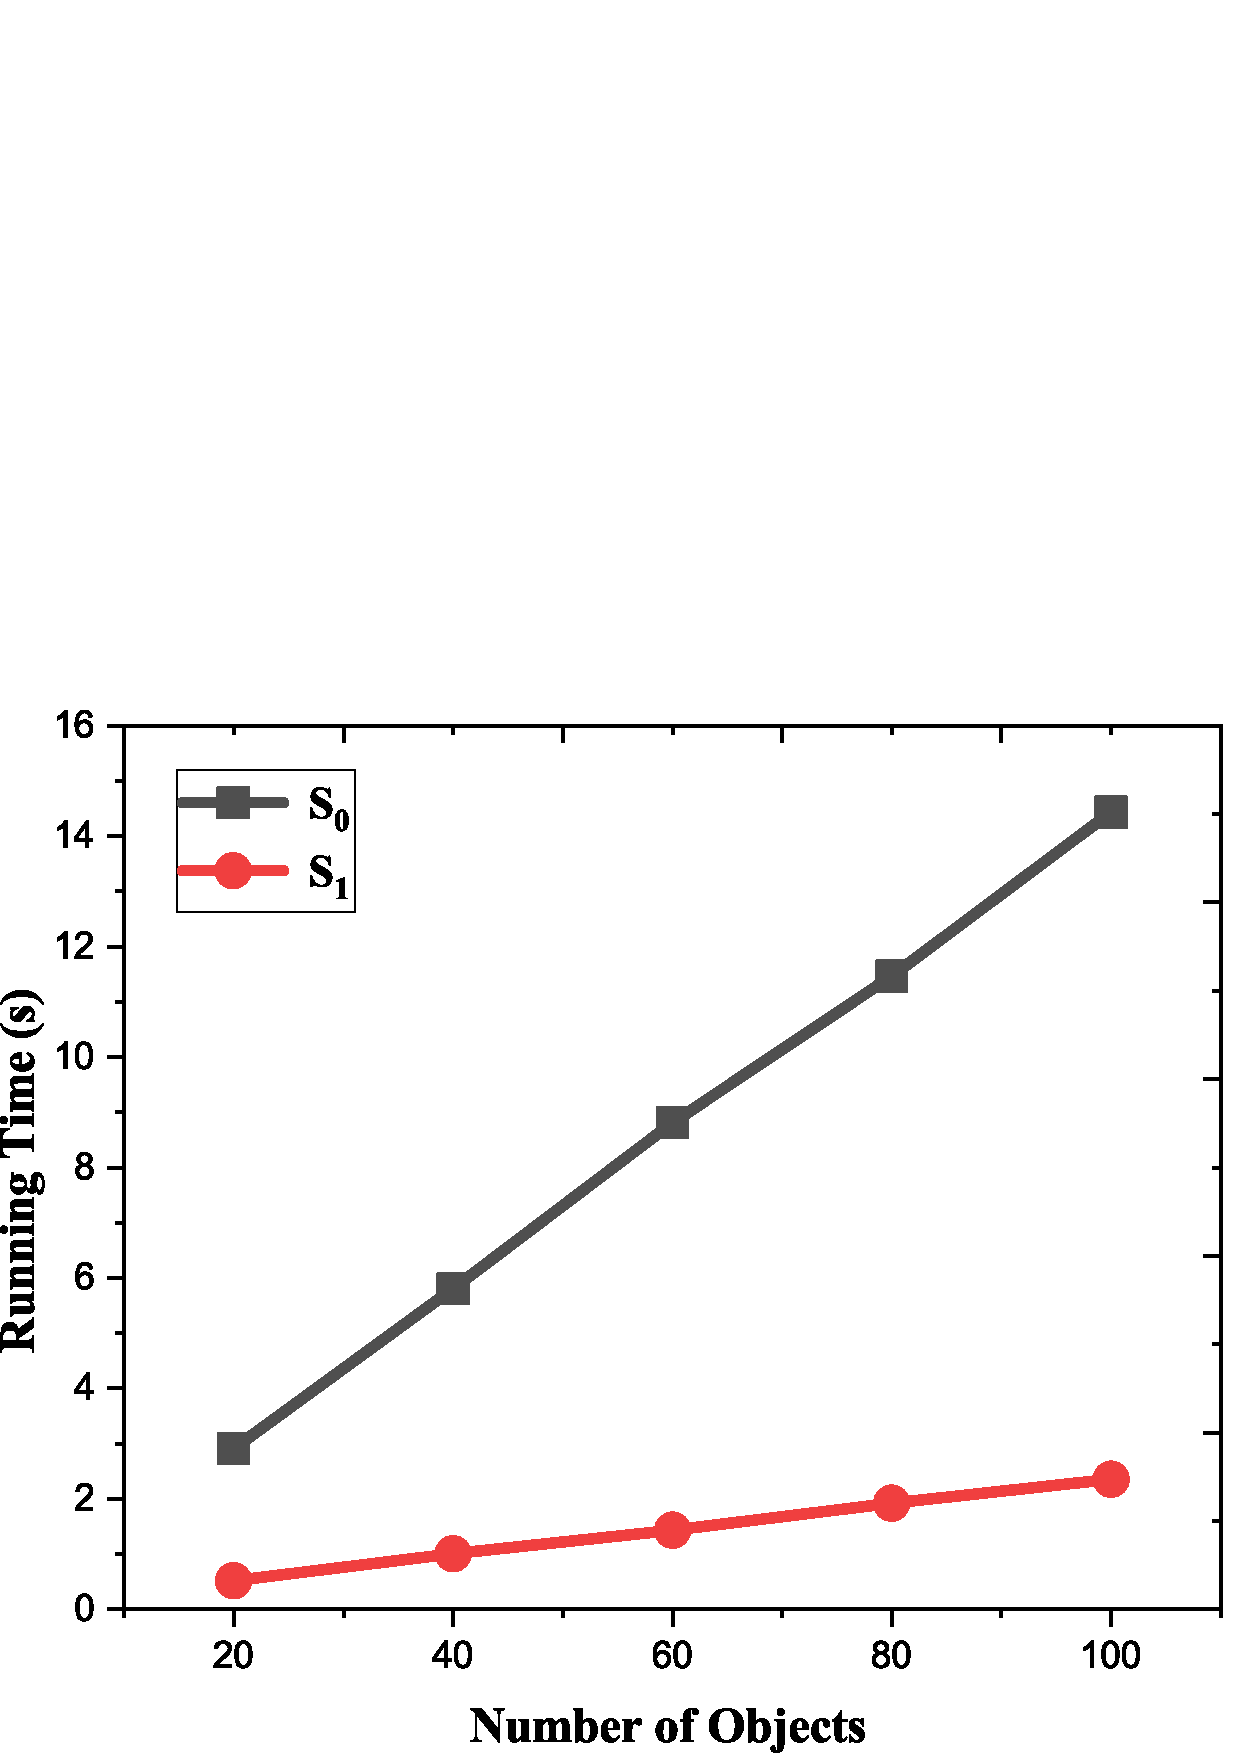
\includegraphics[width=0.48\linewidth]{figures/time_obj.pdf}}
  \subfloat[$M = 20$]{ 
    \label{fig:comp2} 
    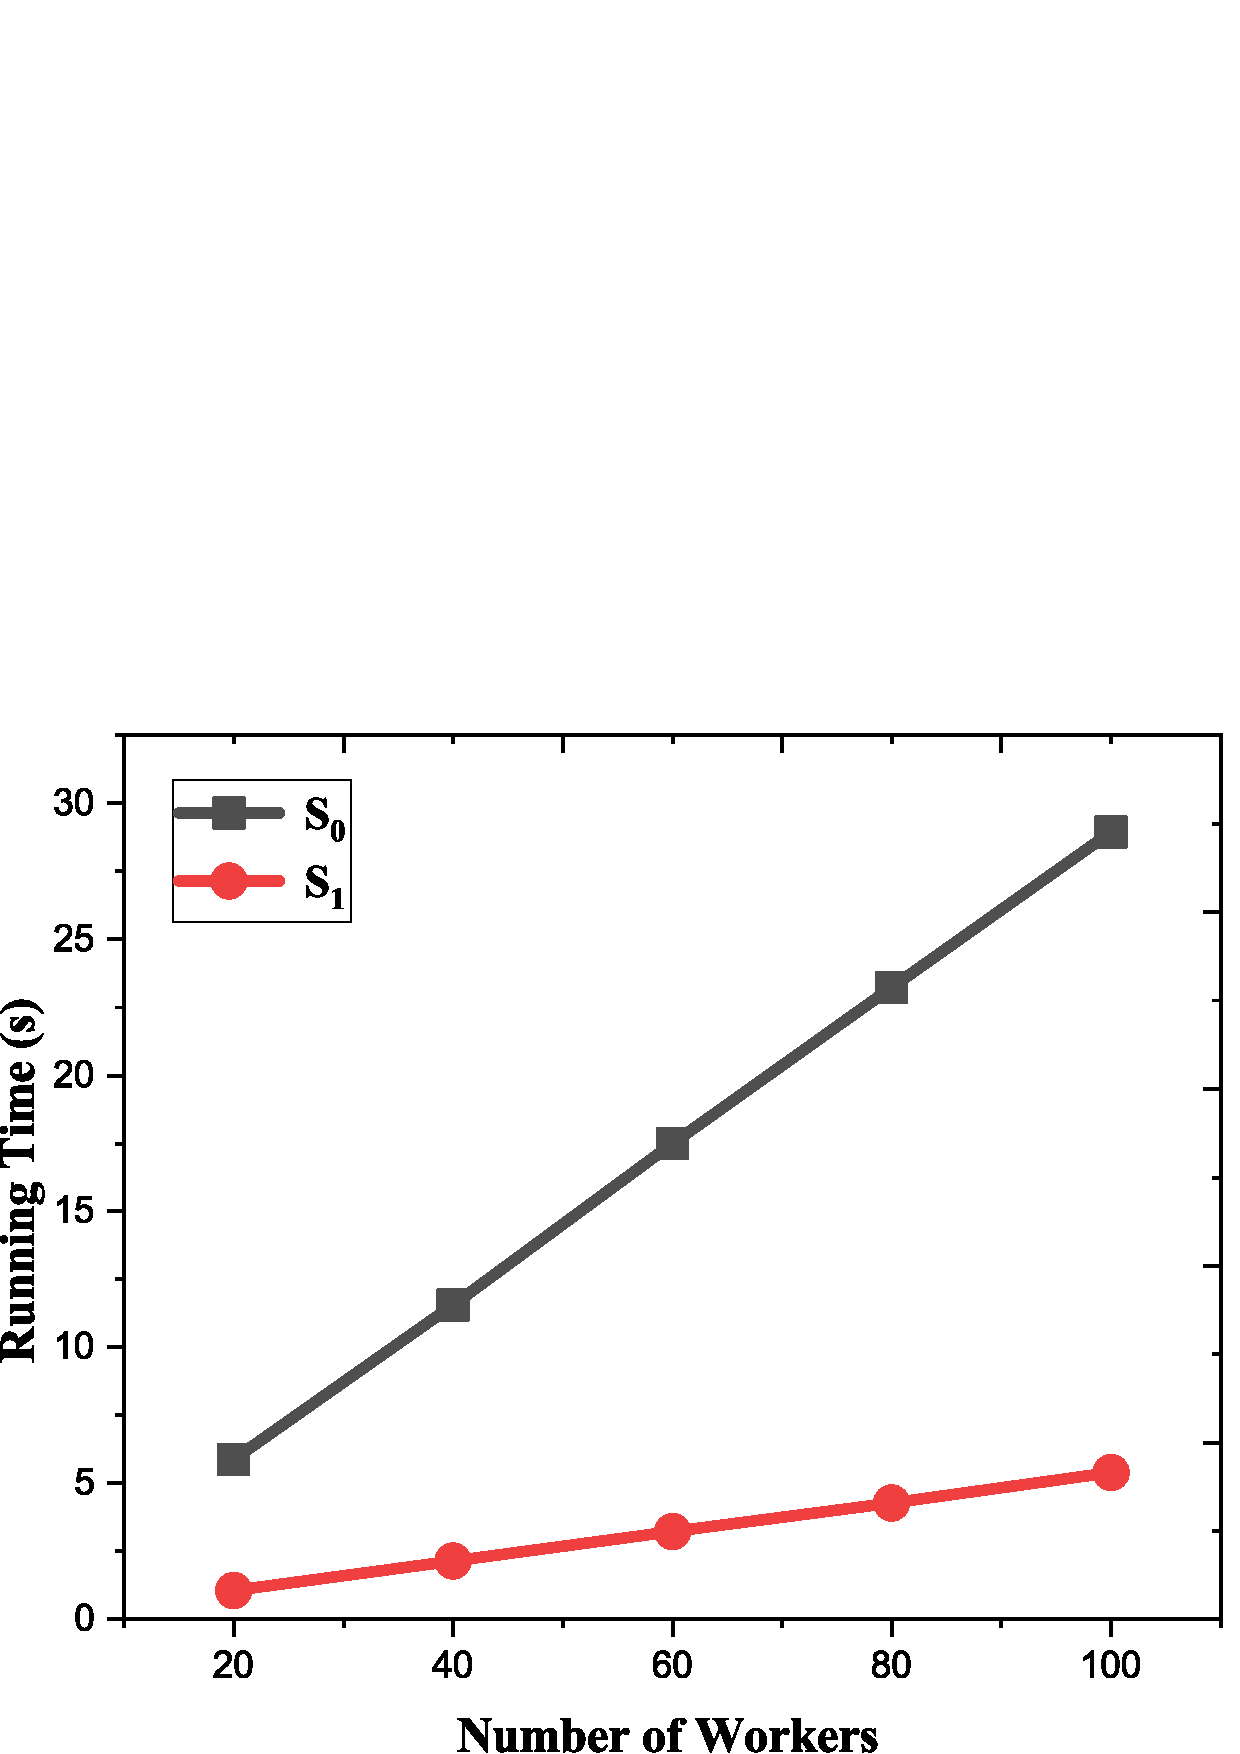
\includegraphics[width=0.48\linewidth]{figures/time_work.pdf}} 
  \caption{Computation Overhead for Each Iteration}
  \label{fig:comp} 
\end{figure}

\begin{table}[!ht]
  \centering
  \caption{Communication Overhead (KB)}~\label{tab:communication}
  \linespread{1.3}\selectfont
  \begin{adjustbox}{max width=0.46\textwidth}
  \begin{tabular}{l l c c c c}
    \hline
    \hline
    \multicolumn{2}{c}{\multirow{2}*{Number of Workers and Objects}} &  \multicolumn{1}{c}{Report Phase} & \multicolumn{1}{c}{Pre-Processing Phase} & \multicolumn{2}{c}{Iteration Phase} \\
    \cmidrule(lr){3-3}\cmidrule(lr){4-4} \cmidrule(lr){5-6} & & Workers to Servers & $S_0$ to $S_1$ & $S_0$ to $S_1$ & $S_1$ to $S_0$ \\
    \hline
    \multirow{3}*{$K=10$} & $M=20$ & 9.60 & 8.08 & 3.44 & 0.04\\
    & $M=40$ & 19.20 & 16.08 & 6.80 & 0.72\\
    & $M=60$ & 28.80 & 24.08 & 10.16 & 1.04\\
    \cmidrule(lr){1-2}
    \multirow{3}*{$M=20$} & $K=20$ & 19.20 & 16.16 & 6.72 & 0.48\\
    & $K=40$ & 38.40 & 32.32 & 13.28 & 0.64 \\
    & $K=60$ & 57.60 & 48.48 & 19.84 & 0.80 \\
    \hline
    \hline
  \end{tabular}
  \end{adjustbox}
\end{table}

As for the iteration phase, we measure the computation cost of $S_0$ and $S_1$ under different numbers of workers and objects for each iteration.
As shown in Fig.~\ref{fig:comp}, the computation cost for $S_1$ is much less compared to $S_0$ under some conditions.
For the communication overhead, TABLE~\ref{tab:communication} reports the communication overhead for each entity in different phases.
It is clear that the communication overhead in the iteration phase is less than that in the non-iteration phase.
Note that the alternative privacy-preserving truth discovery scheme~\cite{zheng_learning_2018} based on CATD is implemented by GC.
However, the computation cost of GC generation and the communication of GC transmission are huge.
We demonstrate that the computation overhead and communication overhead on the workers' side are lightweight, and the communication overhead between two servers is also acceptable for truth discovery in reality.

\section{Conclusion}\label{sec8}
In this paper, we proposed a privacy-preserving truth discovery scheme targeted for privacy-preserving problems in sparse data scenarios.
Firstly, we carefully discussed the privacy issues for truth discovery when sensory data provided by workers are sparse.
After that, we presented a scheme to guarantee these requirements by utilizing additively homomorphic cryptosystem based on the CATD framework.
Finally, through the analysis of security, our proposed scheme achieves strong privacy protection of workers' sensory data, weights, and indicator vectors simultaneously.
Extensive experiments also indicate that the computation overhead of workers and the communication overhead in the iteration phase are lightweight, which implies that the proposed scheme is practical in real mobile crowdsensing systems.

\section*{Acknowledgment}
This work is supported in part by the National Natural Science Foundation of China under Grant No. 61972371 and Youth Innovation Promotion Association of the Chinese Academy of Sciences (CAS) under Grant No. Y202093.

\bibliographystyle{IEEEtran}
\bibliography{ref}

\vspace{12pt}

\end{document}